\ifx\allfiles\undefined
\documentclass[UTF8]{ctexart}
\title{知识准备}
\author{邹远春}
\date{}
\usepackage{xeCJK}
\usepackage{graphicx, subfig}
\usepackage{caption}
\usepackage{listings}
\usepackage{verbatim}
\begin{document}
\maketitle
\else
\chapter{知识准备}
\fi
\section{RLP}

https://github.com/ethereum/wiki/wiki/RLP

\subsection{Definition}

\subsection{Examples}

\subsection{RLP~decoding}

\section{MPT}

以太坊MPT详解

https://blog.csdn.net/weixin\_41545330/article/details/79370198

\begin{figure}
	\centering
	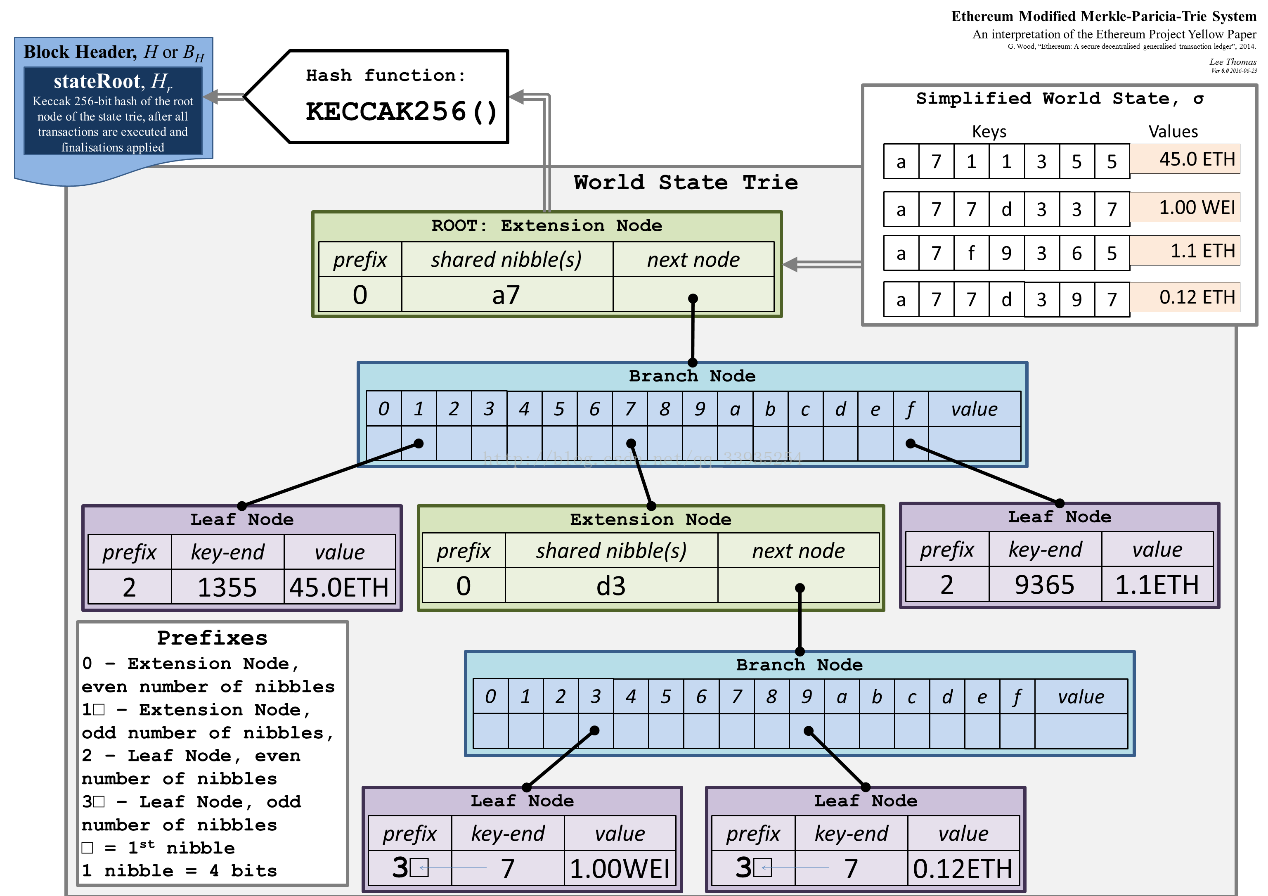
\includegraphics{rlp.png}
	\caption{MTP}
	\label{rlp}
\end{figure}

\section{矿池}

\section{矿机}

\section{世界状态}

\section{分叉}

\section{侧链}

RootStock

\section{闪电网络}

\section{隔离见证}

\section{智能合约}

\section{跨链}

\subsection{公证人}
Notary schemes

\subsection{侧链/中继}
Sidechains/relays

BTC-Replay

Cosmos

Polkadot

\subsection{哈希锁定}
Hash-locking

HTLC

\section{预言机Oracle}

\section{Sharding}

\section{中心化交易所}

\section{去中心化交易所}

\section{钱包}

\subsection{热钱包}

\subsection{冷钱包}

\subsection{硬件钱包}

\subsection{分层确定性钱包}

\section{ERC20}

\section{ERC721}

\section{安全}
形式化证明

\ifx\allfiles\undefined
\end{document}
\fi